\documentclass[a4paper]{article}
\usepackage{graphicx} % Required for inserting images
\usepackage{physics}
\usepackage[margin=2cm]{geometry}
\usepackage[italian]{babel}
\usepackage{siunitx}
\usepackage{float}
\usepackage{hyperref}
\usepackage[shortlabels]{enumitem}
\sisetup{separate-uncertainty=true}
\hypersetup{hidelinks, linktoc=all}
\usepackage{subfig}
\usepackage{changepage}
\usepackage[toc,page]{appendix}
\usepackage{breqn}

\renewcommand\thesubfigure{\arabic{subfigure}}

\sisetup{per-mode=symbol}

\title{\textbf{Lenti}}
\author{Agostino Luca, Cafaro Alessandro, Gili Francesco, Gros Jacques Matteo\\ Turno AII - Gruppo 7\\A.A. 2024-2025}
\date{\today}

\begin{document}
    
\maketitle

\tableofcontents
\newpage

\section{Obiettivi della misura}
    Verificare la validità delle leggi sulle lenti sottili, misurandone le proprietà geometriche; in particolare:
    \begin{enumerate}
        \item Ricavare la distanza focale e l'ingrandimento di una lente biconvessa
        \item Ricavare la distanza focale di una lente piano-convessa
        \item Ricavare la distanza focale di una lente divergente
        \item Misurare la posizione dell'immagine di un sistema di due lenti convergenti non a contatto.
    \end{enumerate}
\section{Apparato sperimentale}
    \begin{itemize}
        \item Banco ottico (sensibilità: \SI{1}{\mm})
        \item Proiettore con illuminazione regolabile
        \item Diapositiva da proiettare
        \item Lenti di diverso tipo: biconvessa, piano-convessa, biconcava
        \item Schermo per visualizzare l'immagine
        \item Calibro (sensibilità: \SI{0.05}{\mm})
    \end{itemize}
    Abbiamo scelto di utilizzare come incertezza della scala graduata del banco ottico il valore di \SI{2}{\mm}, al posto della sua sensibilità, perché meglio rappresentativo della nostra precisione nell'effettuare la misurazione. D'ora in poi, dunque, quando si farà riferimento alla sensibilità dello strumento, si intenderà quella da noi ad esso associata.
\section{Presa dati}
    \subsection{Lente biconvessa}\label{sec:biconvessa}
        Abbiamo fissato la lente biconvessa su un supporto posto a distanza $p=\SI{140(2)}{\mm}$. Successivamente abbiamo compiuto 70 misure ripetute della posizione dell'immagine, spostando lo schermo finché questa non risultasse nitida, con l'accortezza di alternare destra e sinistra come direzioni di avvicinamento.
        %Dati.

        Ci aspettiamo che i due fuochi abbiano la stessa distanza dalla lente; l'abbiamo quindi ruotato di $\pi$ e ripetuto le misure utilizzando la stessa procedura e le medesime accortezze.

        Per entrambe le lenti abbiamo poi calcolato l'ingrandimento come il rapporto tra la distanza di due punti distinti sullo schermo e degli stessi sulla diapositiva.
        %Dati
        
    \subsection{Lente piano-convessa}    
    Abbiamo ripetuto le precedenti misurazioni su una lente convergente piano-convessa mantenendo inalterato il numero di misure e la procedura utilizzata.
    
    \subsection{Lente biconcava}
    Riutilizzando la lente biconvessa della Sezione \ref{sec:biconvessa}, costruiamo un sistema ottico formato da quest'ultima e da una lente negativa biconcava, montandole in modo che siano il più possibile vicine tra loro. Poniamo le due lenti a distanza $p$ dall'oggetto, ed esattamente nello stesso modo descritto precedentemente, misuriamo ripetutamente $q$.
    
    \subsection{Sistema di lenti}
    Utilizzando due lenti convergenti disposte non a contatto, abbiamo misurato 10 volte il valore di $q_2$, ossia la distanza dalle lenti che rende nitida l'immagine sullo schermo.
\section{Analisi dati}
    \subsection{Lente biconvessa}
    Poiché abbiamo compiuto $N=70$ misure ripetute della stessa grandezza, ci aspettiamo che i dati si distribuiscano secondo un andamento gaussiano. Abbiamo dunque eseguito un fit dell'istogramma delle frequenze assolute dei dati.
    \begin{figure}[H]%
    	\centering
    	\subfloat[\centering Lente biconvessa]{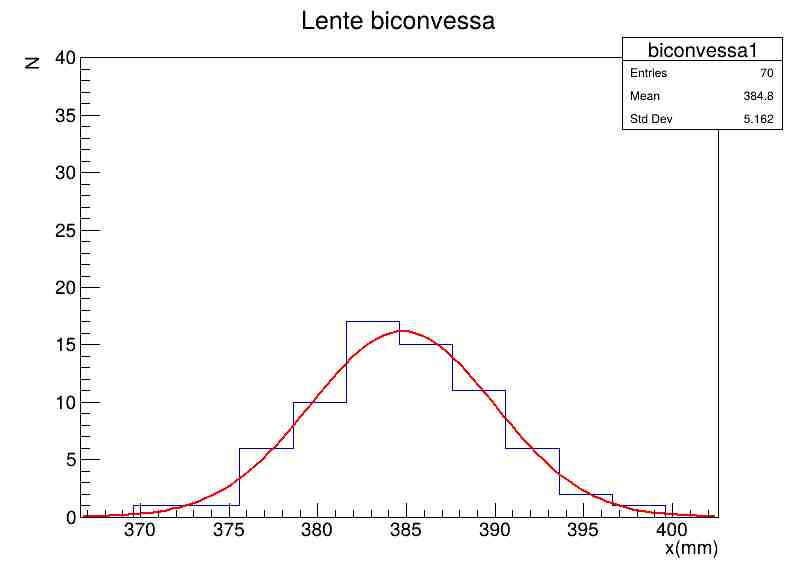
\includegraphics[width=0.4\textwidth]{histo1.jpg}}%
    	\qquad
    	\subfloat[\centering Lente biconvessa ruotata]{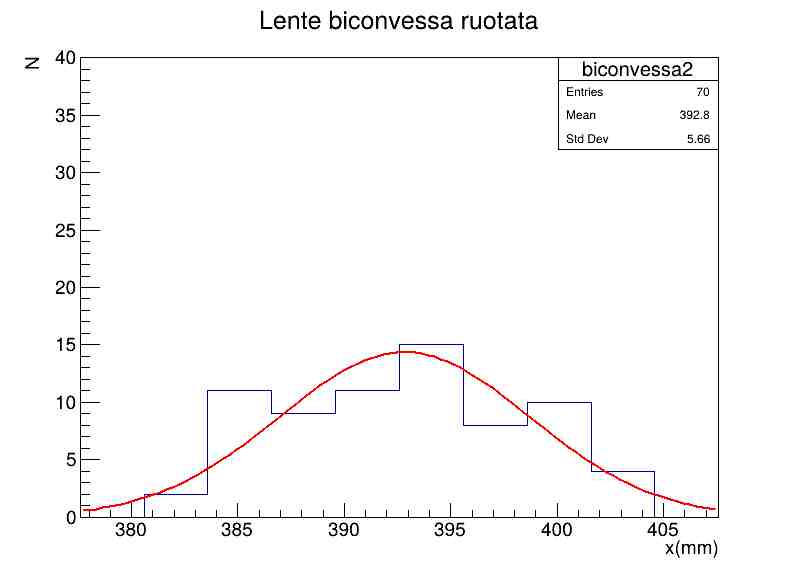
\includegraphics[width=0.4\textwidth]{histo2.jpg}}%
    \end{figure}
    Di seguito riportiamo il test del $\chi^2$, con un livello di significatività del $5\%$:
    \[
    H_0: \text{la distribuzione gaussiana ben descrive quella dei dati sperimentali.}
    \]
    \begin{table}[H]
    	\centering
    	\begin{tabular}{|c|c|c|}
    		\hline
    		 & (1) & (2) \\ \hline
    		$\chi^2$ & 1.942 & 11.010 \\
    		$\nu$ & 9 & 7 \\
    		$\chi^2_c$ & 16.919 & 14.067 \\
    		$\chi^2_s$ & 3.325 & 2.167 \\ \hline
    	\end{tabular}
    	\label{tab:chi-quadro-biconvessa}
    \end{table}
    Nel caso (1) il chi-quadro risulta essere \textit{sospetto} ($\chi^2\leq\chi^2_s$); accettiamo l'ipotesi nulla per i seguenti motivi:
    \begin{itemize}
    	\item % da fare
    \end{itemize}Nel caso (2) il chi-quadro è \textit{accettabile} ($\chi^2\leq\chi^2_c$), dunque accettiamo l'ipotesi $H_0$.
    
    Siccome il fit gaussiano ben descrive la distribuzione dei dati, possiamo considerare $\bar{q} = \mu$:
    \begin{align*}
    	q_1 = \SI{385(2)}{\mm} && q_2 = \SI{393(2)}{\mm}
    \end{align*}
    
    dove come incertezza associata abbiamo tenuto la sensibilità dello strumento, in quanto la deviazione standard della media era inferiore.
    
    Successivamente abbiamo calcolato il valore del fuoco:
    \begin{align*}
    	f_1=\frac{p_1\cdot q_1}{p_1+q_1}=\SI{103(1)}{\mm} && f_2=\frac{p_2\cdot q_2}{p_2+q_2}=\SI{103(1)}{\mm}
    \end{align*}
    Come ci aspettavamo, le due distanze focali sono compatibili.
    
    L'ingrandimento vale invece:
    \begin{align*}
    	G_1=\frac{q_1}{p_1}=\SI{2.75(4)}{} && G_2=\frac{q_2}{p_2}=\SI{2.81(4)}{}
    \end{align*}
    Per verificare che il secondo ingrandimento sia compatibile con il rispettivo valore misurato, abbiamo effettuato un test di Gauss:
    \[
    H_0: \text{abbiamo estratto $G_2-G_{2m}$ da una distribuzione normale centrata intorno a $\mu=0$ con $\sigma=\sqrt{\sigma_{G_2}^2+\sigma_{G_{2m}}^2}=0.07$}
    \]
    \begin{table}[H]
    	\centering
    	\begin{tabular}{|c|c|}
    		\hline
    		z osservato ($z_o$) & 1.75 \\
    		livello di significatività ($\alpha$) & 5\% \\
    		z critico ($z_c$) & 1.96 \\ \hline
    	\end{tabular}
    	\label{tab:gauss-1}
    \end{table}
    Poiché $z_o\leq z_c$, accetto l'ipotesi nulla $H_0$ con un livello di significatività del 5\%.
    \subsection{Lente biconcava}
    \subsection{Sistema di lenti}
\section{Risultati e osservazioni conclusive}
    \subsection{Lente biconvessa}
    \subsection{Lente biconcava}
    \subsection{Sistema di lenti}
\begin{appendices}
    \section{Dati}
    \section{Calcoli}
\end{appendices}
\end{document}
